

% ================================================================
						%1. Introduction
%================================================================
\section{Introduction}
\subsection{Purpose}
The purpose of this document is to describe a demonstration system that explores using an additional HUD mounted MEMS IRU to meet previous installation standards while reducing costs. This system will further be described by its use of sensor data to dynamically find alignment offset error during flight as a consequence to airframe droop. This document describes the hardware and software requirements along with the functional and non-function requirements of the project. This document is intended to be used by the Head-Up display system engineer team of Rockwell Collins as a proof of concept. 

\subsection{Scope}
This project aims to develop a demonstration system to work as a proof of concept for Rockwell Collins. This project is called the HUD Alignment System. The primary goal of this project will be to use sensor data to find the initial alignment offset after HUD installation. The alignment offset must be found within the same accuracy of the previous installation standards and will be used within the system as a hard coded value. The secondary goal will be to use this additional sensor to find the alignment offset during flight to be used within the system as a dynamic value. The dynamic alignment offset must also be found within the desired accuracy standards.\

Currently, the HUD obtains data from an aircraft’s mounted device called inertial reference unit (IRU), this IRU outputs precise and aligned data to the HUD. However, the current alignment process requires specialized equipment and epoxy which is time consuming, costly, and interrupts production line progress for the original equipment manufacturer. In addition, the resulting HUD alignment, while precise, does not compensate for airframe droop during flight. Rockwell Collins looks forward to a new alignment methodology utilizing an inexpensive microelectromechanical systems (MEMS) IRU mounted onto the HUD to infer alignment data from the aircraft’s precisely mounted and aligned IRU. This project works on a solution that utilizes the data from both the inexpensive MEMS IRU and the aircraft mounted IRU to develop an algorithm, which aims to output precise and aligned data with reduced installation cost.\

The outcome (aligned-data) of this algorithm will compensate the alignment error correctly, and the alignment error should be within a range of one milliradian. The product will make the alignment process more dynamic and less time consuming. The dynamic alignment process also makes this new system compensate for the airframe droop that happens during the flight environment. As well as from the perspective of the industries, this product aims to improve the installation process by reducing cost and time for all parties involved.

\subsection{Definitions, Acronyms, and Abbreviations}
\begin{itemize}
	\item \textbf{HUD}
 	\begin{adjustwidth}{2.5em}{0pt}
 	A Head-Up Display (HUD) is a transparent display placed in front of a pilot’s head position in the cockpit of the aircraft. A HUD presents critical flight information to the pilots during the flight environment by using graphical, numerical and symbolical data \cite{hud}.
 	\\
 	\end{adjustwidth}

	\item \textbf{Airframe Droop}
 	\begin{adjustwidth}{2.5em}{0pt}
	As the center of the aircraft is pushed up due to lift, the nose of the aircraft is pulled down by its weight. The result of these conflicting forces causes a bend in the aircraft \textquotesingle s frame.
	\\
 	\end{adjustwidth}

	\item \textbf{Conformal Attitude}
 	\begin{adjustwidth}{2.5em}{0pt}
	A method of presenting flight information on the HUD. With conformal attitude presentation, the displayed information on the HUD is presented with respect to the real world (outside scene in front of the aircraft), and the presentation is dependent on the head position of the pilot \cite{conformal_atti}.
	\\
 	\end{adjustwidth}

 	\item \textbf{Real-time}
 	\begin{adjustwidth}{2.5em}{0pt}
	In this system, the algorithm should recognize and precisely align the alignment error for IMU output within minimal time (e.g., 500 milliseconds).\\
 	\end{adjustwidth}

 	\item \textbf{IRU/IMU}
 	\begin{adjustwidth}{2.5em}{0pt}
	An Inertial Reference Unit (IRU), sometimes it’s called an Inertial Measurement Unit (IMU) is a device consists of inertial sensors typically including MEMS gyroscopes, accelerometers and compasses. These MEMS sensors measure and provide data of an aircraft \textquotesingle s velocity, acceleration and orientation \cite{iru}.
	\\
 	\end{adjustwidth}

 	\item \textbf{MEMS}
 	\begin{adjustwidth}{2.5em}{0pt}
	An Inertial Reference Unit (IRU), sometimes it’s called an Inertial Measurement Unit (IMU) is a device consists of inertial sensors typically including MEMS gyroscopes, accelerometers and compasses. These MEMS sensors measure and provide data of an aircraft \textquotesingle s velocity, acceleration and orientation \cite{mems}.
	\\
 	\end{adjustwidth}

 	\item \textbf{Accelerometer}
 	\begin{adjustwidth}{2.5em}{0pt}
	An electromechanical device that measures the amount of static acceleration due to gravity, in other word, the rate of change in velocity of the mounted object \cite{accelerometer}.
	\\
 	\end{adjustwidth}

 	\item \textbf{MEMS Gyroscope}
 	\begin{adjustwidth}{2.5em}{0pt}
	An electromechanical device that measures rotational motion/angular velocity, in other word, the speed of rotation of the mounted object \cite{gyroscope}.
	\\
 	\end{adjustwidth}

 	\item \textbf{I2C}
 	\begin{adjustwidth}{2.5em}{0pt}
	The Inter-integrated Circuit (I2C) Protocol is a protocol intended to allow multiple “slave” digital integrated circuits (“chips”) to communicate with one or more “master” chips \cite{i2c}.
	\\
 	\end{adjustwidth}

 	\item \textbf{Alignment Algorithm}
 	\begin{adjustwidth}{2.5em}{0pt}
	The uses of mathematical and logical equations to align the input data from the IRUs based on the data from previous precisely pre-aligned IRUs.
	\\
 	\end{adjustwidth}

 	\item \textbf{Symbology}
 	\begin{adjustwidth}{2.5em}{0pt}
	The use and interpretation of symbols or special characters, in order for representing the corresponding flight data.
	\\
 	\end{adjustwidth}

 	\item \textbf{Milliradian}
 	\begin{adjustwidth}{2.5em}{0pt}
	1 Milliradian (MRAD) = 0.001 radian, approximately 0.057296 degrees.
	\\
 	\end{adjustwidth}

 	\item \textbf{Quaternion}
 	\begin{adjustwidth}{2.5em}{0pt}
	Four-element vector that is used to encode any rotation in a 3D coordinate system.
	\\
 	\end{adjustwidth}

 	\item \textbf{Altitude}
 	\begin{adjustwidth}{2.5em}{0pt}
	A distance measurement (usually in vertical) between ground and the aircraft.\\
 	\end{adjustwidth}

 	\item \textbf{Latitude}
 	\begin{adjustwidth}{2.5em}{0pt}
	AAn angular distance shown as a horizontal line, in degrees, minutes, and seconds of a point north or south of the Equator. Lines of latitude are often referred to as parallels \cite{latAndLong}.
	\\
 	\end{adjustwidth}

 	\item \textbf{Longitude}
 	\begin{adjustwidth}{2.5em}{0pt}
	An angular distance shown as a vertical line, in degrees, minutes, and seconds, of a point east or west of the Prime (Greenwich) Meridian. Lines of longitude are often referred to as meridians \cite{latAndLong}.
 	\end{adjustwidth}
\end{itemize}


\subsection{Overview}
The second section of this document contains an overall description of the product, including the product perspectives, product functions, user characteristics, constraints, assumptions and dependencies. The third section of this document will specify the project’s requirements. 




% ================================================================
							% 2. Overall Description 
% ================================================================
\newpage
\section{Overall Description}
\subsection{Product Perspective}
Currently, the HUD’s position is precisely aligned and determined during installation by a mechanical alignment method. Since the product will be developed as a proof of concept, this product will be a demonstrated system by using two separate MEMS IMUs respectively simulate for the add-on “HUD” IRU and “Aircraft” IRU. By including the “HUD” IRU, this alignment system will be able to determine the HUD’s position as well as providing additional benefit to determine the HUD’s shifting position during flight as a result of airframe droop.


\subsection{Product Functions}
\begin{itemize}
	\item 
	Both ”HUD” and “Aircraft” IRUs will measure the acceleration and orientation of the mounted target object.
	\item 
	The master boards (microcontrollers) will recognize both IRUs’ measurement data (raw) and output to the alignment algorithm.
	\item 
	The alignment algorithm will compare the outputs from both IRUs (data from the “aircraft” IRU is assumed to be precise and aligned) and be able to quantify the alignment error as well as their correlation.
	\item 
	The alignment algorithm will be able to calculate the target object’s precise position based on the acceleration and orientation output from both IRUs.
	\item 
	The algorithm will account for the target object’s position and rotation to ensure that the conformal attitude, flight path information and other displayed data is accurately aligned.
	\item 
	This algorithm will determine the alignment error to a desired accuracy level as 1.0 milliradian.
	\\
\end{itemize}
See figure 1 as the entire workflow for data transmission and connections between the hardware

\begin{figure}[!ht]
  \centering
      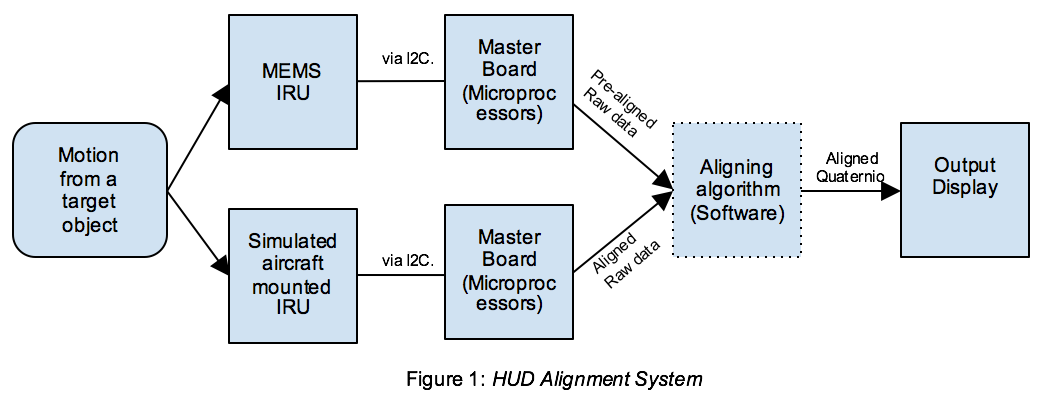
\includegraphics{diagram}
\end{figure}


\subsection{User Characteristics}
This alignment algorithm is intended to be applied to the HUD system, which will be used by Rockwell Collins to determine the availability of having an additional MEMS IRU in the for the new HUD alignment system. The intended users of this product are the technical expertise in this area, such as HUD system engineers in Rockwell Collins. The audience of this document will be familiar with the abbreviations and jargon used to describe the product. This familiarity reduces the requirement for more elaborate explanations of the project. As our expected user maintains technical expertise in the field, they will expect our project to meet a higher standard of competence.


\subsection{Constraints}
\textbf{Hardware Limitations:} 
\begin{itemize}
	\item 
	This IMU model will be SparkFun MPU-9250 IMU MEMS sensors. 
	\item 
	The SparkFun MPU-9250 IMU is programmable to output 8,000 samples per second, down to 3.9 samples per second,
	\item 
	The microcontroller model will used as the Metro Mini 328 chip to set up the sensors.   
	\item 
	The model ATmega328P as the core chip in Metro Mini 328. 
	\item 
	The algorithm will account for the target object’s position and rotation to ensure that the conformal attitude, flight path information and other displayed data is accurately aligned.
	\item 
	This algorithm will determine the alignment error to a desired accuracy level as 1.0 milliradian.
	\\
\end{itemize}

\textbf{Signal Handshake Protocol:}
\begin{itemize}
	\item 
	I2C protocol is used to communicate between IMU MEMS IMUs.
	\\
\end{itemize}

\textbf{Higher order language Requirement:}
\begin{itemize}
	\item 
	C/C++ programming language is used for the development of the software. 
\end{itemize}

\subsection{Assumption and Dependencies}
\begin{itemize}
	\item 
	This product will depend on both the microcontroller and the sensors that are being used within the system in terms of hardware limitations.
	\item 
	We assume that the microcontroller can interact with our sensors as well as to meet any other hardware concerns.
	\item 
	We assume that the sensors are sufficient to simulate the aircraft IRU and HUD mounted MEMS IRU when building our demonstration system.
	\\\\
\end{itemize}



% ================================================================
						% 3. Specific Requirements
% ================================================================

\section{Specific Requirements}
\subsection{External Interface Requirements}
This section describes the detailed breakdown of the entire system. A description of the user, hardware, software and communication interfaces are presented.

\subsubsection{User Interface}
Our user interface will be the physical manipulation of our demonstration system in order to generate movement data.The software user interface for this project is a display that will show the properly aligned symbology of the airplane. A generic HUD symbology picture which could be moved up/down, left/right will be used to illustrate the alignment.
\\

\subsubsection{Hardware Interface}
\begin{itemize}
	\item 
	A microcontroller will have access to data from two separate 9-axis sensors that are used to represent the aircraft IRU and HUD mounted MEMS IRU.
	\item 
	The microcontroller will additionally be connected to an output device.
	\item 
	The hardwares are still not decided at this point. However, these are the product that we might use for the hardwares. 
	\item 
	Product Name: Metro Mini 328 - 5V 16MHz \cite{trinket}
	\item 
	Features: 
	\begin{itemize}
		\item ATmega328P onboad chip in QFN package
		\item 16MHz clock rate, 28K FLASH available
	\end{itemize}	
	\item 
	IMU Model: SparkFun IMU Breakout - MPU-9250 \cite{mpu9250}
	\item 
	Features: 
	\begin{itemize}
		\item Digital-output X-, Y-, and Z-axis angular rate sensors (gyroscopes) with a user-programmable full-scale range of ±250, ±500, ±1,000 and ±2,000°/sec and integrated 16-bit ADCs

		\item Digital-output triple-axis accelerometer with a programmable full-scale range of ±2g, ±4g, ±8g and ±16g and integrated 16-bit ADCs

		\item 3-axis silicon monolithic Hall-effect magnetic sensor with magnetic concentrator

		\item Digitally programmable low-pass Gyroscope filter
		\item Gyroscope operating current: 3.2mA
		\item Accelerometer normal operating current: 450µA
		\item Magnetometer normal operating current: 280µA at 8Hz repetition rate
		\item VDD supply voltage range of 2.4 – 3.6V
		\\
	\end{itemize}	
\end{itemize}


\subsubsection{Software Interface}
At this point we are still not sure what additional library/software we will use in this project. We will use C-like language (C/C++) to program this project on Arduino IDE. We will also use the ATmega328P library since we will use the ATmega328P chip as our microcontroller board.
\\
\subsubsection{Communication Interface}
I2C protocol will be used to communicate with MPU-9250 and Metro Mini 328. 


%3.2
\subsection{Functional Requirements}
\subsubsection{Sensors}

\paragraph{Sensor recognition}
This program will have the capability to recognize sensors. This program shall recognize and identify all sensors provided to the system. This functionality is the core to the input recognition capability.
\\
\paragraph{Input recognition}
This program will correctly interpret the data provided by the recognized sensors. This program will have the ability not only to recognize the outputs from the sensors, but also to interpret the outputs so it can be used as a proper input for the program. This functionality will be dependent on the success of the sensor recognition functionality.
\\
\subsubsection{Algorithm}
\paragraph{Quaternion Manipulation}
This program will have the ability to do quaternion manipulation to the inputs. Inputs that are received from the sensors will be compared and manipulated to determine the alignment error. The desired accuracy level of the alignment error is within one milliradian. This functionality will execute in real-time, within 500 milliseconds.
\\
\subsubsection{Statistics}
\paragraph{Statistical Corelation}
This program will have the capability to generate a confidence interval for each alignment error output being generated by the algorithm. Outputs in a form of alignment error will be used to determine the confidence interval of the data. This functionality will execute in real-time, within 500 milliseconds. 
\\
\subsubsection{Simulation}
\paragraph{Simulated HUD}
This program will have the capability to display the properly aligned symbology of the airplane. A generic HUD symbology picture which could be moved up/down, left/right will be used to illustrate the alignment of the airplane.


%3.3
\subsection{Performance Requirements}
\begin{itemize}
	\item Number of terminals to be supported: Two terminals for both MEMS sensors. 
	\item Amount of information to be handled: Programmable up to 3.9 to 8000 data per seconds. We will start with 10 data per seconds from both sensors. 
	\item Type of information to be handled: Quaternion 
	\item Valid Range of Accuracy: milliradians 
	\item Timing: Currently not specified 
	\item Destination of Output: Simulated HUD interface
\end{itemize}	

%3.4
\subsection{Design Constraints}
This product is limited to the specification of the hardware. This product will get its input from MEMS IRU and aircraft IRU. The specification of the MEMS IRU and “aircraft” IRU will alter the quaternion manipulations being done to the data.  Different MEMS IRUs will require a different quaternion manipulations to achieve the expected standard of accuracy. This hardware dependability makes this product dependent to one specific hardware. Thus, limiting our design to one specific hardware.

Another design constaint is to precisely get the hardware error from the IMU sensors, since the alignment algorithm requires high accuracy data input, minor error may cause unexpected offset of the final results. Therefore, we will need a feasible experiment to test and measure the sensor error precisely.

%3.5
\subsection{Software System Attributes}
\subsubsection{Reliability}
It is important to make sure the system in both software and hardware will be able to run properly and smoothly without abortion. As a proof a concept, reliability is important, a wrong data will lead to incorrect outcome in the determination of further development that based on this products.
\\
\subsubsection{Availability}
The software piece of the entire system should be able to run without any crashes or other situation lead to system error (this is a critical issue during an real flight situation). Yet, the hardware pieces should be able to detect the failed components at the time when it happens.This product will have the capability to detect error and may restart itself when crashes.
\\
\subsubsection{Security}
This product will be used internally by Rockwell Collins and since this product will be used for a proof of concept, security is not an issue.
\\
\subsubsection{Maintainability}
This system does not work solely as a software neither a hardware product, which it has to be tested onto real flight situation. The current development  is for a proof of concepts. Hence, maintainability will not be an issue for this project. This project will be used as a reference and basis of a future project in Rockwell Collins, but not directly used as the core/underlying code for any long-term product.
\\
\subsubsection{Portability}
Portability of this system exists on the hardware level. Since hardware programming is required for this project to manipulate functionalities of the hardware components (e.g., sensors, microprocessors/microcontrollers), specific hardware programming language for this project is host-dependent. It depends on the specific controller boards we are using. In this project, we are using C-like languages (C/C++), which is one of the proven portable language for hardware programming for most general microcontrollers/microprocessors, therefore this system has high portability.







